\documentclass[a4paper,10pt]{article}
\usepackage[a4paper, total={6in, 8in}]{geometry}
\setlength\parindent{0pt}
\usepackage[utf8]{inputenc}
\usepackage{graphicx} 
\usepackage{amsmath}
\usepackage{amsfonts}
\usepackage{amssymb}
\usepackage{listings}
\usepackage{ragged2e}
\usepackage{listings}
\usepackage{color}
\usepackage[table]{xcolor}
\usepackage{soul}
\setlength{\parskip}{\baselineskip}%
\setlength{\parindent}{0pt}%

\begin{document}
\begin{titlepage}
	\centering
	
\includegraphics[width=.6\textwidth]{liu-logo.png}\par
	\vfill
	{\scshape\Large TDDE01 MACHINE LEARNING\par}
	{\huge\bfseries Lab 1 - B18 Group Report\par}
	\vspace{0.5cm}
    {\large\itshape Lawrence Thanakumar Rajappa (lawra776)\\
     \large\itshape Grégoire Vola (grevo149)\\
     \large\itshape Kyriakos Domanos (kyrdo817)\par}
	\vfill
	{\large \today\par}
\end{titlepage}
\definecolor{dkgreen}{rgb}{0,0.6,0}
\definecolor{gray}{rgb}{0.5,0.5,0.5}
\definecolor{mauve}{rgb}{0.58,0,0.82}

\lstset{frame=tb,
  language=R,
  aboveskip=3mm,
  belowskip=3mm,
  showstringspaces=false,
  columns=flexible,
  basicstyle={\small\ttfamily},
  numbers=none,
  numberstyle=\tiny\color{gray},
  keywordstyle=\color{blue},
  commentstyle=\color{dkgreen},
  stringstyle=\color{mauve},
  breaklines=true,
  breakatwhitespace=true,
  tabsize=3
}
\textbf{\underline{Our group work methodology}} \par
In our group, we all 3 were working on different systems, so we got different results.
We communicated our results in the end by using the university system. Even if our results are slightly different, we are getting to the same conclusions.
For example, in the 1\textsuperscript{st} assignment, we found different confusion matrices but the misclassification rates were roughly the same.

We worked on the questions separately and helped each other on the questions we had trouble to solve. In general, we had more trouble with assignment 2 and some comprehension problem.

In the end, we all 3 gathered to compare our results and wrote the group report, as well as discussing the matters that put us in the most difficulty. \par
\vspace{0.5cm}
\textbf{\underline{Assignment 1}} \par
We have created logistic regression model for Spambase data in Linux environment and got the following 
Confusion Matrices and Misclassification rates Which are same for all three of us. \par
2. Confusion Matrix and Misclassification Rate for p$>$0.5 \par
\begin{center}
	\textbf{Confusion Matrix} \par
	\begin{tabular}{|c|c|}
		\hline
		Confusion Matrix - Training Data&
		Confusion Matrix - Test Data\\
		\hline
		\cellcolor{yellow!100} 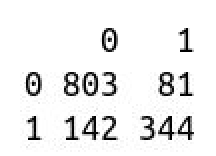
\includegraphics[width=25mm,scale=0.10]{Confusion_Matrix_training_Data_1.png} &
		\cellcolor{yellow!100} 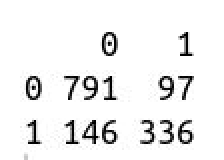
\includegraphics[width=25mm,scale=0.10]{Confusion_Matrix_test_Data_1.png}\\
		\hline
\end{tabular}\par \par
	\textbf{Misclassification Rate} \par
	\begin{tabular}{|c|c|}
		\hline
		Misclassification Rate - Training Data&
		Misclassification Rate - Test Data\\
		\hline
		\cellcolor{yellow!100} 0.1627737 $\sim$ 16.277\% & \cellcolor{yellow!100} 0.1773723 $\sim$ 17.737\%\\
		\hline
	\end{tabular}\par
\end{center} \par
Our model is doing a relatively good job at predicting the results for our test data with a ~82.3\% accuracy. The accuracy is a bit higher at predicting the results for our train data, ~83.7\% , which is to some extend expected since these data were used for training our model.\par
\newpage
3. Confusion Matrix and Misclassification Rate for p$>$0.8 \par
\begin{center}
	\textbf{Confusion Matrix} \par
	\begin{tabular}{|c|c|}
		\hline
		Confusion Matrix - Training Data&
		Confusion Matrix - Test Data\\
		\hline
		\cellcolor{yellow!100} 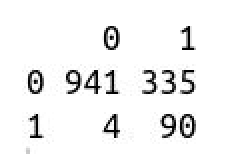
\includegraphics[width=25mm,scale=0.10]{Confusion_Matrix_training_Data_2.png} &
		\cellcolor{yellow!100} 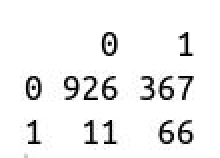
\includegraphics[width=25mm,scale=0.10]{Confusion_Matrix_test_Data_2.png}\\
		\hline
	\end{tabular}\par \par
	\textbf{Misclassification Rate} \par
	\begin{tabular}{|c|c|}
		\hline
		Misclassification Rate - Training Data&
		Misclassification Rate - Test Data\\
		\hline
		\cellcolor{yellow!100} 0.2474453 $\sim$ 24.744\% & \cellcolor{yellow!100} 0.2759124 $\sim$ 27.591\%\\
		\hline
	\end{tabular}\par
\end{center} 
The new rule has increased the Misclassification rates for both training and test dataset. This is because of the 
threshold or probability limit which was set. In 0.5 probability scenario, the data points which are above this 
threshold line was classified as 1 and the data points below the line was classified as 0. But, when the threshold
was increased to 0.8, the points which were actually observed as 1, was classified as 0, hence the Misclassification
rate has increased and also the accuracy has reduced from 82\% to 72\%.\par
\vspace{0.5cm}
We have created KNN model for the same Spambase dataset with different K values in Linux environment. 
We have got same confusion Matrices and Misclassification rates which are given below \par
4. Misclassification Rate when k = 30 \par
\begin{center}
	\textbf{Confusion Matrix} \par
	\begin{tabular}{|c|c|}
		\hline
		Confusion Matrix - Training Data&
		Confusion Matrix - Test Data\\
		\hline
		\cellcolor{yellow!100} 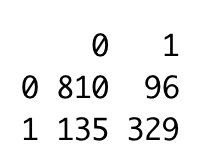
\includegraphics[width=25mm,scale=0.10]{Confusion_Matrix_knn_training_Data_1.png} &
		\cellcolor{yellow!100} 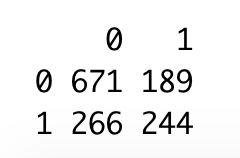
\includegraphics[width=25mm,scale=0.10]{Confusion_Matrix_knn_test_Data_1.png}\\
		\hline
	\end{tabular}\par \par
	\textbf{Misclassification Rate} \par
	\begin{tabular}{|c|c|}
		\hline
		Misclassification Rate - Training Data&
		Misclassification Rate - Test Data\\
		\hline
		\cellcolor{yellow!100} 0.1686131 $\sim$ 16.861\% & \cellcolor{yellow!100} 0.3321168 $\sim$ 33.211\%\\
		\hline
	\end{tabular}\par
\end{center}\par
By comparing step 4 and step 2, we could see that there is a huge difference in correct predictions and Misclassification rates.
Logistic Regression model with p $>$ 0.5 suits very well for this dataset rather than knn. \par
\vspace{0.5cm}
5. Misclassification Rate when k = 1 \par
\begin{center}
	\textbf{Confusion Matrix} \par
	\begin{tabular}{|c|c|}
		\hline
		Confusion Matrix - Training Data&
		Confusion Matrix - Test Data\\
		\hline
		\cellcolor{yellow!100} 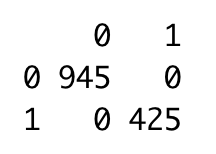
\includegraphics[width=25mm,scale=0.10]{Confusion_Matrix_knn_training_Data_2.png} &
		\cellcolor{yellow!100} 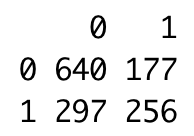
\includegraphics[width=25mm,scale=0.10]{Confusion_Matrix_knn_test_Data_2.png}\\
		\hline
	\end{tabular}\par \par
	\textbf{Misclassification Rate} \par
	\begin{tabular}{|c|c|}
		\hline
		Misclassification Rate - Training Data&
		Misclassification Rate - Test Data\\
		\hline
		\cellcolor{yellow!100} 0 $\sim$ 0\% & \cellcolor{yellow!100} 0.3459854 $\sim$ 34.598\%\\
		\hline
	\end{tabular}\par
\end{center}
In terms of \textit{\textbf{Bias-Variance trade off}}, if K = 1, then the training data will have low bias hence it behaves
well with training data. But, it fails to generalize the testing data and it will increase test data prediction error and 
leads to high variance. Low Bias and high variance leads to overfitting. Hence KNN model with K = 1 is not an admissible
model to use. \hl{In the last lab group report, we have used \textbf{\textit{kknn()}} function, hence we got weird results. But,
when we used \textbf{\textit{train.kknn()}} function, we got the expected results.}
\par
\vspace{0.5cm}
\textbf{\underline{Assignment 2}} \par
2. Based on the probability model, P(x$|$$\theta$) = $\theta$e\textsuperscript{-$\theta$x}, we can see that
this data belongs to exponential distribution. We have used the below formula to calculate log-likelihood
\par
\begin{center}
	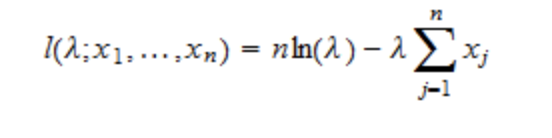
\includegraphics[width=50mm,scale=0.10]{Log-likelihood-formula.png}
\end{center}
and plotted the below graph and the maximum likelihood value of $\theta$ is 1.12 \par
\begin{center}
	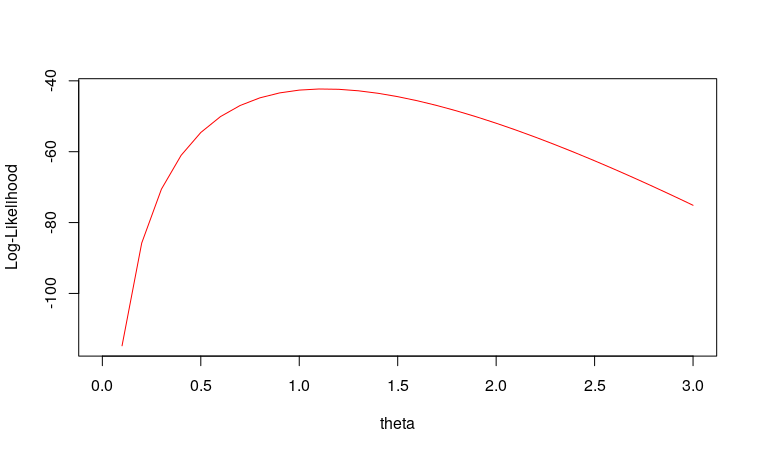
\includegraphics[width=.5\textwidth]{log-likelihood-full-data.png}
\end{center}
3. By using the same function but with only 6 set of observations, we have generated the plot which is given below,\par
\begin{center}
	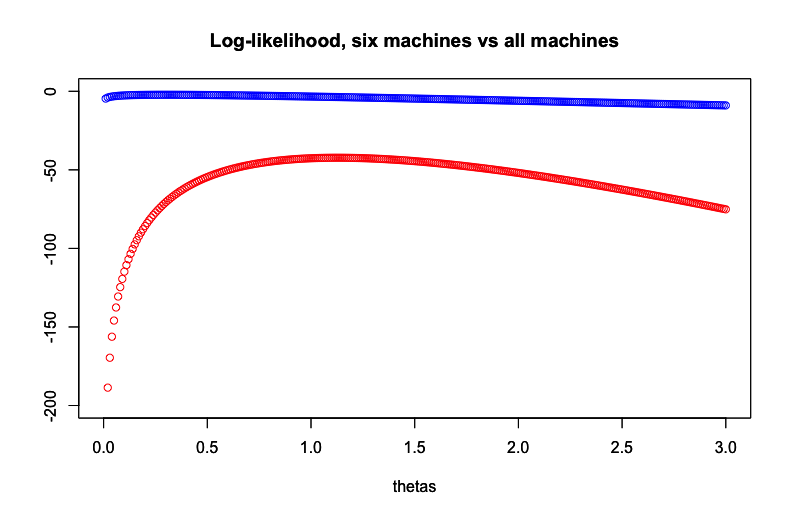
\includegraphics[width=.5\textwidth]{Log-likelihood.png}
\end{center}
From the plot we can see that, blue curve is unreliable as it is using only first 6 observations of the data and we will
miss out information. Eventhough blue plot has higher $\theta$, reliability is worse when data points are limited.
\hl{The maximum log-likelihood value of $\theta$ is 1.126217 for full set of observations and 1.785681 for first 6
observations.}\par 
\vspace{0.5cm}
\par
4. By using bayesian model p(x$|$$\theta$) = $\theta$e\textsuperscript{-$\theta$$x$} and a prior p($\theta$) = $\lambda$e\textsuperscript{-$\lambda$$\theta$}
and also $\lambda$ = 10, we need to compute the function \textit{l}($\theta$) = log(p(x$|$$\theta$)p($\theta$)). 
We have created the above-mentioned function in R and generated the plot by using the values returned by the 
above function which is given below. \par
\begin{center}
	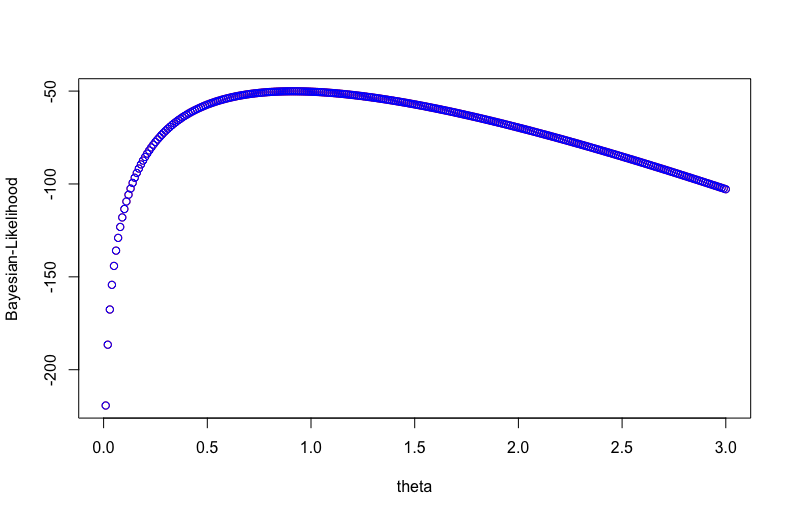
\includegraphics[width=.5\textwidth]{Bayesian.png}
\end{center}
\hl{The maximum likelihood value of $\theta$ is 0.91 compared to previous 1.12. This is used to measure how good the model fits the data.}
\par
\newpage
5. \begin{center}
	\begin{tabular}{|c|c|}
		\hline
		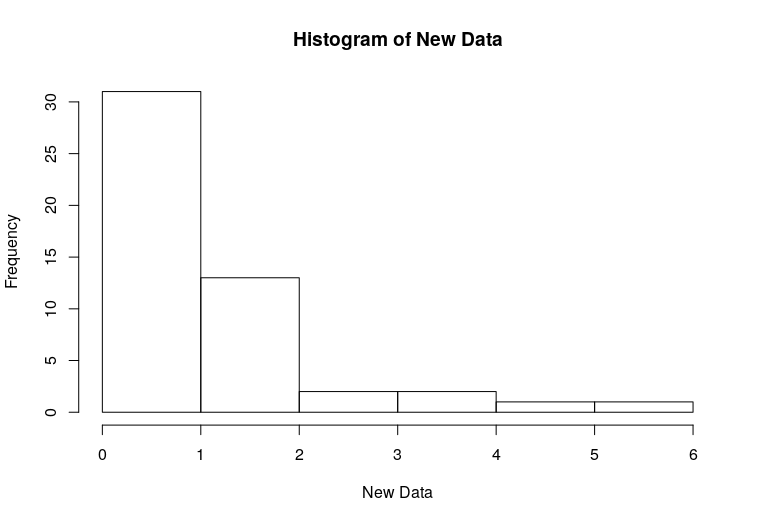
\includegraphics[width=.5\textwidth]{Hist_New_Data.png}&
		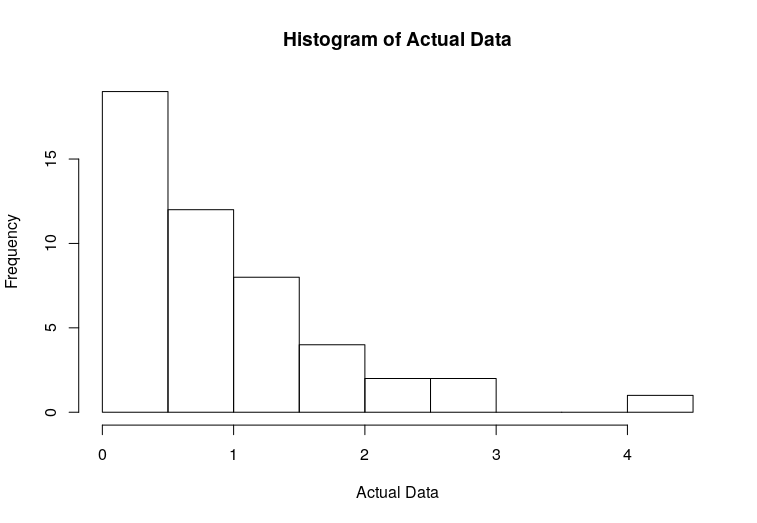
\includegraphics[width=.5\textwidth]{Hist_Actual_Data.png}\\
		\hline
	\end{tabular}\par
\end{center} \par
From the above histograms, we can conclude that both histograms looks similar and follows exponential distribution and
chosen model is a good model. \par
\vspace{0.5cm}
\textbf{\underline{Assignment 4}} \par
1. Plot of Moisture VS Proteins
\begin{center}
    \setlength{\arrayrulewidth}{1.0pt}
    \begin{tabular}{|c|}
        \hline
		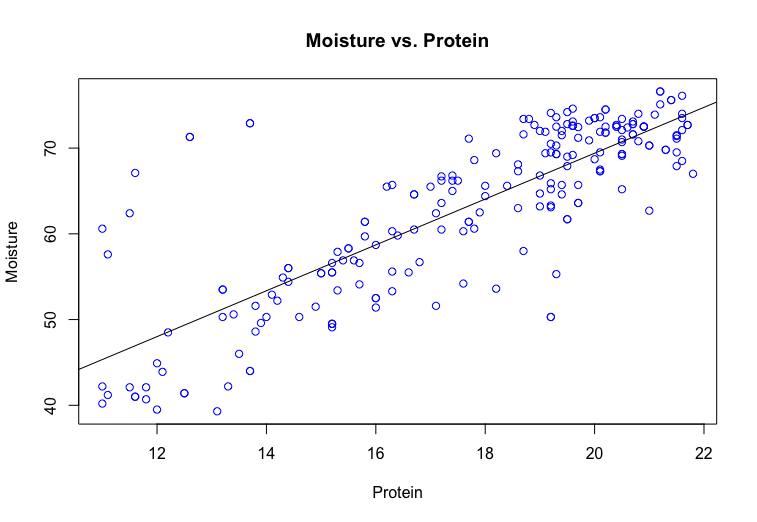
\includegraphics[width=.5\textwidth]{assignment_4_1.png}\\
		\hline
    \end{tabular}
\end{center}
From the scatter plot, we can observe that there is a linearly increasing relationship between \textbf{'Moisture'} and
\textbf{'Protein'} variables by a smoothing line. Moreover, linear regression concept is to have a linear relationship
between response variable and dependent variables. \par
\vspace{0.5cm}
2. Now, let us consider a model m\textsubscript{i} where moisture is normally distributed and expected moisture is
a polynomial function of protein. The probabilistic model is given below \par
\begin{center}
	independent variable (X) = Protein\\
	dependent variable (Y) = Moisture\\
	Y $\sim$ M\textsubscript{0}+M\textsubscript{1}*x+M\textsubscript{2}*x\textsuperscript{2}+........+M\textsubscript{n}*x\textsuperscript{n}
\end{center} \par
\hl{MSE would be a better criterion in order to determine which model is best based on lower MSE.}
\par
\vspace{0.5cm}
3. MSE
\begin{center}
    \setlength{\arrayrulewidth}{1.0pt}
    \begin{tabular}{|c|}
        \hline
		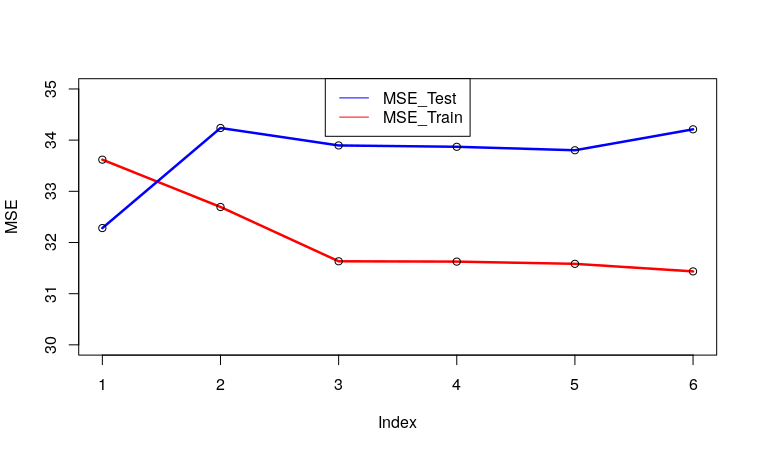
\includegraphics[width=.5\textwidth]{MSE_Train_Test.png}\\
		\hline
    \end{tabular}
\end{center}\par
The above plot describes the training error and testing error for tecator dataset. We can observe that as the polynomial
degrees increases, the MSE for test set increases and lower MSE for training set. In terms of Bias-Variance
trade off, as the model complexity increases because of increase in polynomial degree, there is a high variance on training
data and hence this will have higher error rates on test data as well as training set has low bias. Low Bias and High Variance
leads to overfitting while training and the model performs poorer on test dataset.\hl{Based on the plot, \textbf{model\_3} would
be a better model when compared with other models, as it has optimum training and testing error when compared with other models.}
\par
\vspace{0.5cm}
4. Now, we need to use stepAIC function in R for a variable selection on a linear model where \textit{Fat} is response variable
and \textit{channel1-channel100} is independent variables. After running the function stepAIC, we get a total 63 variables which are given below,
\begin{center}
    \setlength{\arrayrulewidth}{1.0pt}
    \begin{tabular}{|c|}
        \hline
		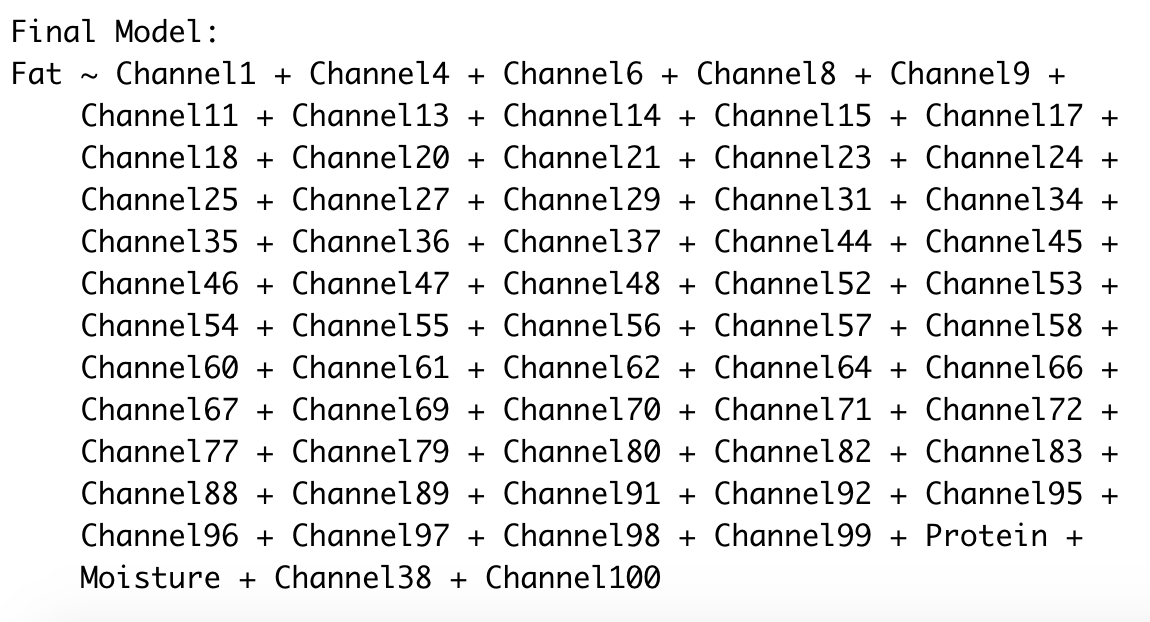
\includegraphics[width=.5\textwidth]{Variable_Selection.png}\\
		\hline
    \end{tabular}
\end{center}
\vspace{0.5cm}
\newpage
5. Now, we have applied Ridge regression to the scaled independent and the dependent variables, as values to be scaled
before applying Ridge regression on them. Ridge regression is applied by using the glmnet function in R.
The coefficients dependency on log of penalty factor $\lambda$ is given below,\\
\begin{center}
    \setlength{\arrayrulewidth}{1.0pt}
    \begin{tabular}{|c|}
        \hline
		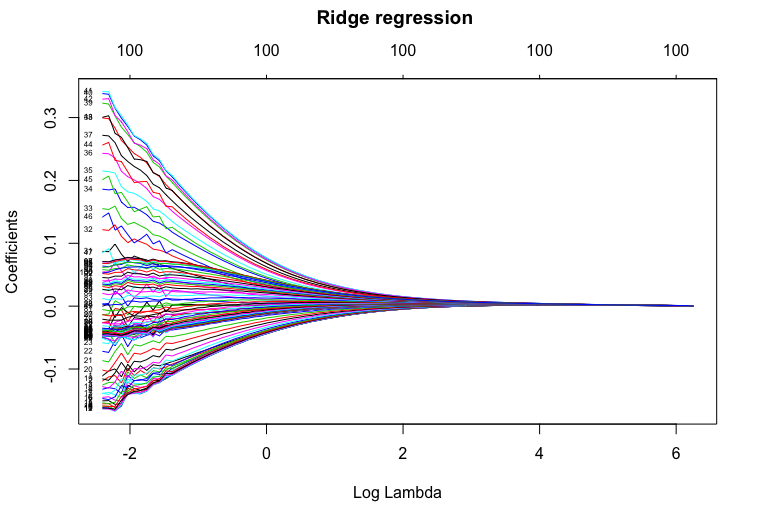
\includegraphics[width=.5\textwidth]{Ridge_Regression.png}\\
		\hline
    \end{tabular}
\end{center}\par
From the above graph, we can say that, if $\lambda$ increases, all coefficients go to zero.It is a small difference, but as per Ridge regression the coefficients go towards 0, but they don't reach 0. \par
\vspace{0.5cm}
\par
6. We do the same but it is for Lasso Regression,
\begin{center}
	\setlength{\arrayrulewidth}{1.0pt}
    \begin{tabular}{|c|}
        \hline
		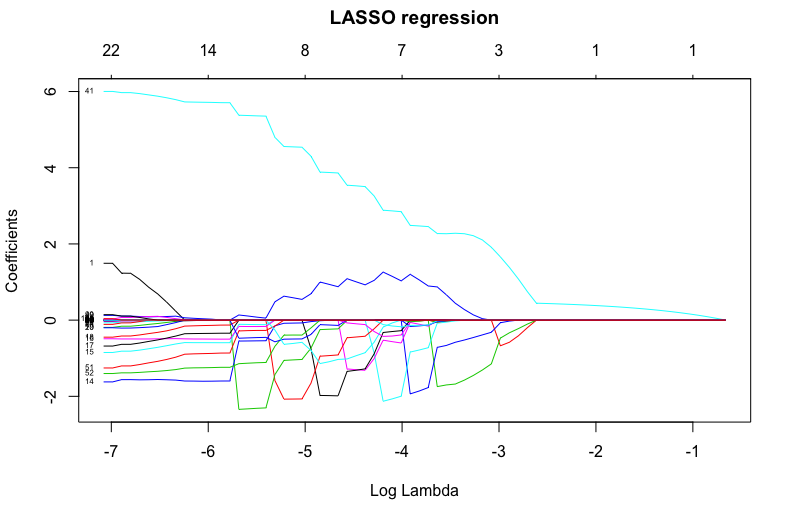
\includegraphics[width=.5\textwidth]{Lasso_Regression.png}\\
		\hline
    \end{tabular}
\end{center}
\par
From the above graph we can see that, most of the features have bigger impact and some of the features are completely 
ignored. In the plot above we can also see that as the $\lambda$ increases, the coefficients go to 0 in contrast to the Ridge regression which was close to 0. Additionally we can see that in comparison to the Ridge regression we now have much less coefficients. LASSO regression is a little better at simplifying models as it can exclude variables that are not useful, however that advantage applies only when there are variables that are not useful. \par
\vspace{0.5cm}
\newpage
7. Now, we need to use cross-validation and find optimal LASSO Model. The plots are given below,
\begin{center}
	\setlength{\arrayrulewidth}{1.0pt}
    \begin{tabular}{|c|}
        \hline
		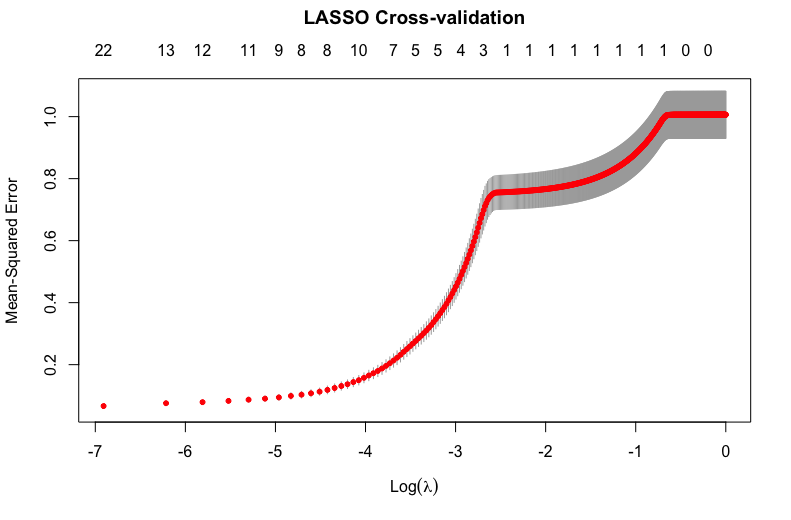
\includegraphics[width=.5\textwidth]{Lasso_Cross_Validation.png}\\
		\hline
    \end{tabular}
\end{center}
\par
By interpreting the plot, we conclude that optimal $\lambda$ value is 0. The number of features selected were 22 
according to the plot for that specific lambda value. Moreover, LASSO gives lesser MSE than stepAIC eventhough, stepAIC
selected 63 features than LASSO. 
In conclusion, it is not always better to use more features while modeling but at the same time it depends on the 
dataset and the number of features in the dataset.
\par
\vspace{0.5cm}
\huge \textbf{\emph{\underline{Code Appendix}}} \par
\large \textit{\textbf{Assignment 1}} \par
\begin{lstlisting}
library(readxl) #Library to read spreadsheet based files
library(kknn) #Library to implement KNN algorithm
options(scipen=999) #To avoid scientific notations
RNGversion('3.5.1')
#Assignment 1
#Reading from excel file
data = read_excel("spambase.xlsx",sheet = "spambase_data")
#1. Splitting the data
n=dim(data)[1]
set.seed(12345)
id=sample(1:n, floor(n*0.5))
#Converting target variable "Spam" to factor
data$Spam = as.factor(data$Spam)
train=data[id,]
test=data[-id,]


#2. Logistic Regression with P(Y|X)>0.5
logisticModel_1 = glm(Spam~.,family = binomial,data = train)
summary(logisticModel_1)

#Function to calculate misclassification rate
missclass=function(actualData,predictedData){
  n=length(actualData)
  return(1-sum(diag(table(actualData,predictedData)))/n)
}

#0.5 classification principle
predicted_training_prob_1 = predict(logisticModel_1,newdata = train,type="response")
predicted_training_1 = ifelse(predicted_training_prob_1>0.5,1,0)
table(as.factor(predicted_training_1),train$Spam)
missclass(train$Spam,as.factor(predicted_training_1))

predicted_test_prob_1 = predict(logisticModel_1,newdata = test,type = "response")
predicted_test_1 = ifelse(predicted_test_prob_1>0.5,1,0)
table(as.factor(predicted_test_1),test$Spam)
missclass(test$Spam,as.factor(predicted_test_1))

#0.8 classification principle
predicted_training_prob_2 = predict(logisticModel_1,newdata = train,type="response")
predicted_training_2 = ifelse(predicted_training_prob_2>0.8,1,0)
table(as.factor(predicted_training_2),train$Spam)
missclass(train$Spam,as.factor(predicted_training_2))

predicted_test_prob_2 = predict(logisticModel_1,newdata = test,type = "response")
predicted_test_2 = ifelse(predicted_test_prob_2>0.8,1,0)
table(as.factor(predicted_test_2),test$Spam)
missclass(test$Spam,as.factor(predicted_test_2))


#3. KNN

knnModel_1 = train.kknn(Spam~.,data = train,kmax = 30)

predicted_3_training_data = predict(knnModel_1,newdata = train)
table(as.factor(predicted_3_training_data),train$Spam)

predicted_3_testing_data = predict(knnModel_1,newdata = test)
table(as.factor(predicted_3_testing_data),test$Spam)

missclass(train$Spam,as.factor(predicted_3_training_data))
missclass(test$Spam,as.factor(predicted_3_testing_data))

knnModel_2 = train.kknn(Spam~.,data=train,kmax = 1)

predicted_4_training_data = predict(knnModel_2,newdata = train)
table(as.factor(predicted_4_training_data),train$Spam)

predicted_4_testing_data = predict(knnModel_2,newdata = test)
table(as.factor(predicted_4_testing_data),test$Spam)

missclass(train$Spam,as.factor(predicted_4_training_data))
missclass(test$Spam,as.factor(predicted_4_testing_data))

\end{lstlisting}
\par
\vspace{0.5cm}
\large \textit{\textbf{Assignment 2}} \par
\begin{lstlisting}
	#Assignment - 2
	library(readxl) #Library to read spreadsheet based files
	options(scipen=999) #To avoid scientific notations
	set.seed(12345)
	RNGversion('3.5.1')
	#1. Reading the data
	machineData = read_excel("machines.xlsx",sheet = "machines")
	
	#Distribution
	hist(machineData$Length,probability = TRUE,xlab = "Length", main = "Length Vs Density")
	lines(density(machineData$Length),col="blue", lwd=2)
	
	#Log-likelihood function
	theta = seq(from=0,to=3,by=0.01)
	logLikelihood = function(theta,dataVector)
	{
	  return(length(dataVector)*log(theta)-theta*sum(dataVector))
	}
	
	maximumLikelihood = function(theta,dataVector)
	{
	  return(length(dataVector)/sum(dataVector))
	}
	
	plot(theta, logLikelihood(theta,machineData$Length), ylim = c(-200,0), col = 'red', xlab="thetas", ylab = "",
		 main="Log-likelihood, six machines vs all machines")
	par(new = TRUE)
	plot(theta, logLikelihood(theta,machineData[1:6,]), ylim = c(-200,0), col='blue', xlab="thetas", ylab = "",
		 main="Log-likelihood, six machines vs all machines")
	
	maximumLikelihood(theta,machineData$Length)
	maximumLikelihood(theta,machineData$Length[1:6])
	
	#4.
	bayesian <- function(data, theta,lambda) {
	  return( logLikelihood(theta, data) + log(lambda*exp(-lambda*theta)))
	}
	
	plot(theta,bayesian(machineData$Length,theta,10),col="red",xlab="theta",
		 ylab = "Bayesian-Likelihood")
	par(new=TRUE)
	points(theta,bayesian(machineData$Length,theta,10),col="blue")
	theta[which.max(bayesian(machineData$Length,theta,10))]
	#5.
	theta[which.max(logLikelihood(theta,machineData$Length))]
	new_observation_exp = (rexp(50, theta[which.max(logLikelihood(theta,machineData$Length))]))
	hist(new_observation_exp,main = "Histogram of New Data",xlab="New Data")
	hist(machineData$Length, main = "Histogram of Actual Data",xlab = "Actual Data")
	par(new = TRUE)
	
\end{lstlisting}
\par
\vspace{0.5cm}
\large \textit{\textbf{Assignment 4}} \par
\begin{lstlisting}
	#Assignment - 3
library(readxl) #Library to read spreadsheet based files
library(ggplot2) #For visualisation
options(scipen=999) #To avoid scientific notations
set.seed(12345)
#Loading data
tecatorData = read_excel("tecator.xlsx",sheet = "data")

#1. plotting Moisture VS Protein
plot(tecatorData$Protein, tecatorData$Moisture, main="Moisture vs. Protein",xlab = "Protein",ylab = "Moisture",col="blue")
abline(lm(formula = Moisture ~ Protein, data=tecatorData))

#Subsetting data
requiredData = tecatorData[,103:104]
id = sample(1:nrow(requiredData),floor(nrow(requiredData)*0.5))
train = requiredData[id,]
test = requiredData[-id,]

#Linear Regression
  #M1
tecatorModel_1 = lm(formula = Moisture ~ Protein, data=train)
sm1 = summary(tecatorModel_1)
sm1

  #M2
tecatorModel_2 = lm(formula = Moisture ~ Protein+I(Protein^2), data=train)
sm2 = summary(tecatorModel_2)
sm2

  #M3
tecatorModel_3 = lm(formula = Moisture ~ Protein+I(Protein^2)+I(Protein^3), data=train)
sm3 = summary(tecatorModel_3)
sm3

  #M4
tecatorModel_4 = lm(formula = Moisture ~ Protein+I(Protein^2)+I(Protein^3)+I(Protein^4), data=train)
sm4 = summary(tecatorModel_4)
sm4

  #M5
tecatorModel_5 = lm(formula = Moisture ~ Protein+I(Protein^2)+I(Protein^3)+I(Protein^4)+I(Protein^5), data=train)
sm5 = summary(tecatorModel_5)
sm5

  #M6
tecatorModel_6 = lm(formula = Moisture ~ Protein+I(Protein^2)+I(Protein^3)+I(Protein^4)+I(Protein^5)+I(Protein^6), data=train)
sm6 = summary(tecatorModel_6)
sm6

MSE_train = numeric(6)
MSE_train[1] = mean((train$Moisture-predict.lm(tecatorModel_1,train[,1]))^2)
MSE_train[2] = mean((train$Moisture-predict.lm(tecatorModel_2,train[,1]))^2)
MSE_train[3] = mean((train$Moisture-predict.lm(tecatorModel_3,train[,1]))^2)
MSE_train[4] = mean((train$Moisture-predict.lm(tecatorModel_4,train[,1]))^2)
MSE_train[5] = mean((train$Moisture-predict.lm(tecatorModel_5,train[,1]))^2)
MSE_train[6] = mean((train$Moisture-predict.lm(tecatorModel_6,train[,1]))^2)

MSE_test = numeric(6)
MSE_test[1] = mean((test$Moisture-predict.lm(tecatorModel_1,test[,1]))^2)
MSE_test[2] = mean((test$Moisture-predict.lm(tecatorModel_2,test[,1]))^2)
MSE_test[3] = mean((test$Moisture-predict.lm(tecatorModel_3,test[,1]))^2)
MSE_test[4] = mean((test$Moisture-predict.lm(tecatorModel_4,test[,1]))^2)
MSE_test[5] = mean((test$Moisture-predict.lm(tecatorModel_5,test[,1]))^2)
MSE_test[6] = mean((test$Moisture-predict.lm(tecatorModel_6,test[,1]))^2)

plot(1:6,MSE_train,type="l",ylim = c(20,45),col="red",lwd=2.5,xlab = "Index",ylab = "MSE")
lines(1:6,MSE_test,col="blue",lwd=2.5)
legend(x="center",legend = c("MSE_Test","MSE_Train"),lwd=1,col=c("Blue","Red"),lty=1)


print(anova(tecatorModel_1,tecatorModel_2,tecatorModel_3,tecatorModel_4,tecatorModel_5,tecatorModel_6))

#4. Variable Selection
library(MASS)
aicData = tecatorData
aicData = aicData[,-c(103:104)]
aicData = aicData[,-c(1)]
stepaic = stepAIC(lm(Fat~.,data = aicData))
stepaic$anova

#5. Ridge Regression
library(glmnet)
covariates = scale(tecatorData[, 2:101])
response = scale(tecatorData$Fat)
ridge_model = glmnet(as.matrix(covariates),
                     response, alpha = 0, family="gaussian")
plot(ridge_model, xvar="lambda", label=TRUE, main="Ridge regression \n\n")

#6. Lasso Regression
lasso_model = glmnet(as.matrix(covariates),
                     response, alpha = 1, family="gaussian")
plot(lasso_model, xvar="lambda", label=TRUE, main="LASSO regression\n\n")

#7. Cross-Validation
lasso_model_cv = cv.glmnet(as.matrix(covariates), response, alpha=1, family="gaussian", lambda=seq(0,1,0.001))
plot(lasso_model_cv, xvar="lamdba", label=TRUE, main="LASSO Cross-validation\n\n")
coef(lasso_model_cv, s="lambda.min")
print(lasso_model_cv$lambda.min)
\end{lstlisting}
\end{document}

